\section*{Results}

% In the Results section, you should demonstrate your baseline model’s performance, perfor- mances for each of the parts of Q4.b and Q4.c. You should include both of the performance metrics described in Evaluation metrics (see part 1 above in Implementation Instructions). Please organize these results into a series of concise tables. The formatting is your choice, as long as it is easily interpretable.
% For each architecture include:
% (a) A single plot showing both training and validation loss curves;
% (b) Validation set pixel accuracy and average IoU.
% (c) Visualizations of the segmented output for any one image in the test set along with the original image. Use the color coding mapping in the voc.py for this (Please refer to visualize.ipynb for help on plotting).
\begin{figure}[H]
	\centering
	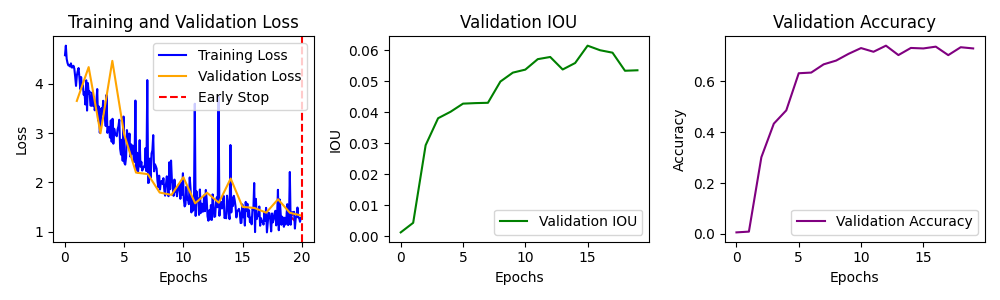
\includegraphics[width=\textwidth]{plots/baseline}
	\caption{Baseline Augmentation}
	\label{fig:baseline}
\end{figure}

\begin{figure}[H]
	\centering
	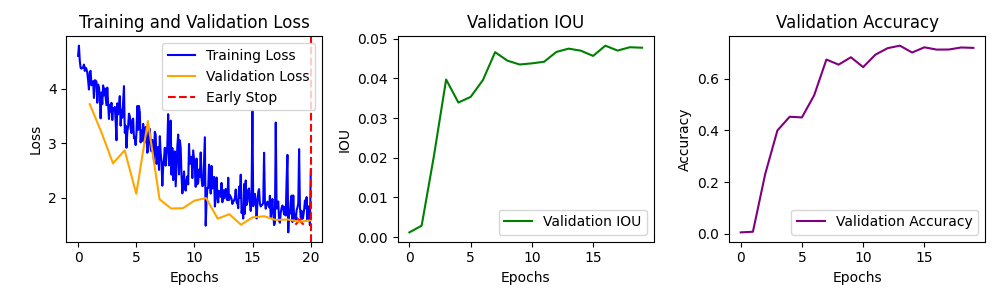
\includegraphics[width=\textwidth]{plots/baseline_augmentation}
	\caption{Baseline Augmentation}
	\label{fig:baseline_aug}
\end{figure}

\begin{figure}[H]
	\centering
	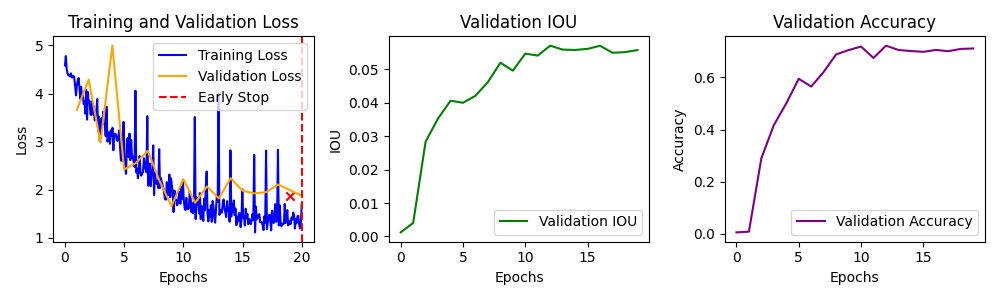
\includegraphics[width=\textwidth]{plots/baseline_cosine}
	\caption{Baseline Cosine}
	\label{fig:baseline_cos}
\end{figure}

\begin{figure}[H]
	\centering
	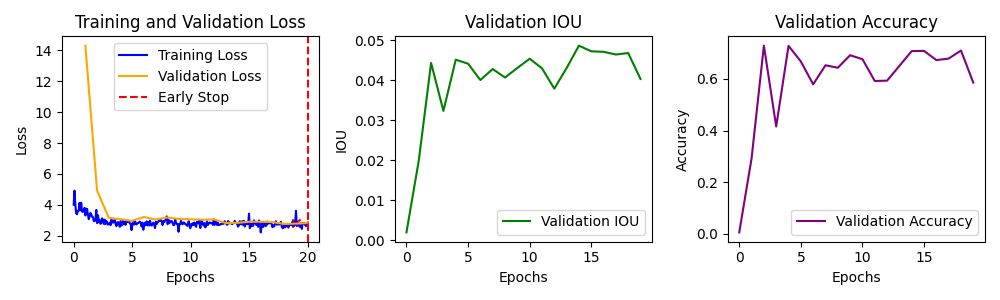
\includegraphics[width=\textwidth]{plots/baseline_weights}
	\caption{Baseline Weights}
	\label{fig:baseline_weights}
\end{figure}

\begin{figure}[H]
	\centering
	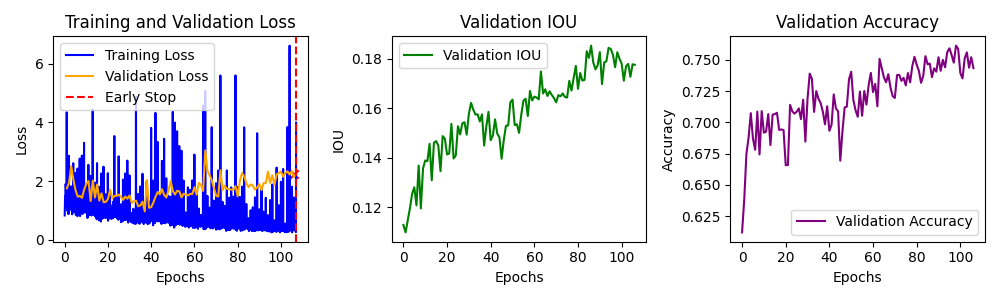
\includegraphics[width=\textwidth]{plots/darrennet_augment_affine}
	\caption{DarrenNet Augment Affine}
	\label{fig:darren_aug_aff}
\end{figure}

\begin{figure}[H]
	\centering
	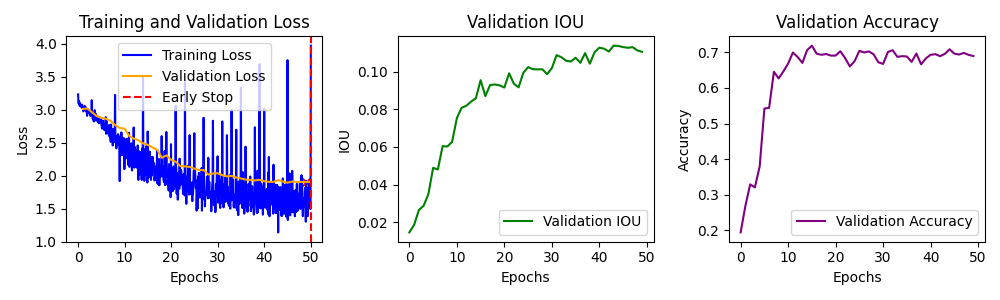
\includegraphics[width=\textwidth]{plots/darrennet_transfer}
	\caption{DarrenNet Transfer}
	\label{fig:darren_transfer}
\end{figure}

\begin{figure}[H]
	\centering
	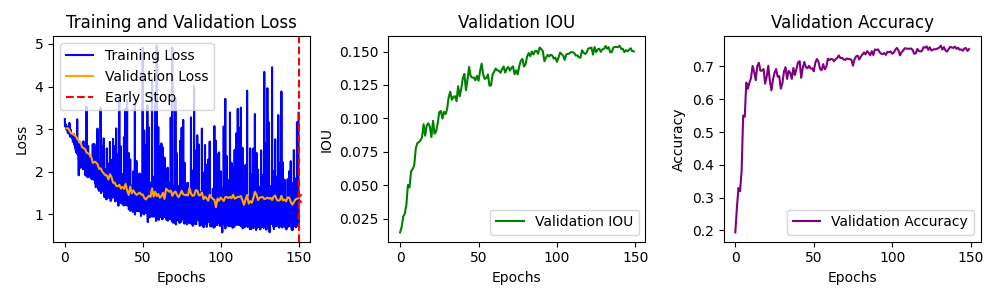
\includegraphics[width=\textwidth]{plots/darrennet_transfer_augment}
	\caption{DarrenNet Transfer Augment}
	\label{fig:darren_transfer_aug}
\end{figure}

\begin{figure}[H]
	\centering
	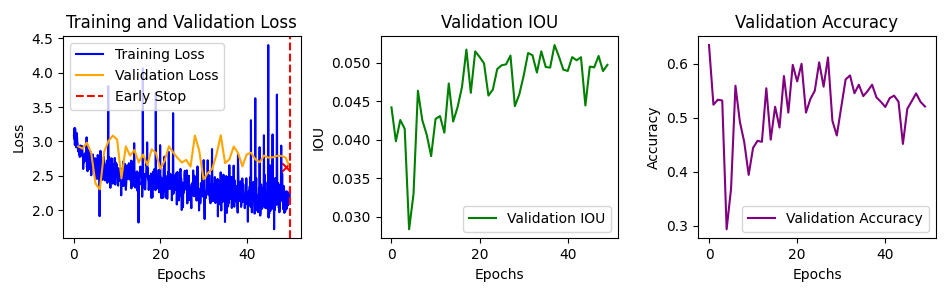
\includegraphics[width=\textwidth]{plots/unet}
	\caption{UNet}
	\label{fig:unet}
\end{figure}

\begin{figure}[H]
	\centering
	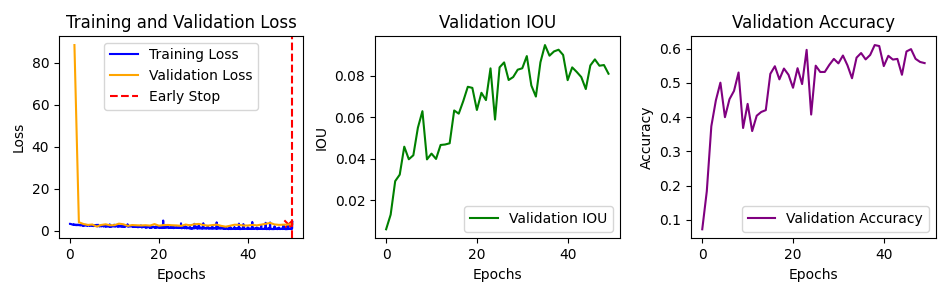
\includegraphics[width=\textwidth]{plots/unet_transfer}
	\caption{UNet Transfer}
	\label{fig:unet_transfer}
\end{figure}
